\chapter{others}
\section{vimrc\ \small(gy)}
	\inputminted{vim}{others/.vimrc}
\section{STL释放内存\ \small(Durandal)}
	\inputminted{cpp}{others/stl_clear.cpp}
\section{开栈\ \small(Durandal)}
	\inputminted{cpp}{others/rsp.cpp}
\section{O3\ \small(gy)}
	\inputminted{cpp}{others/o3.cpp}
\section{读入优化\ \small(ct)}
    \inputminted{cpp}{others/input_optimize.cpp}
\section{Java\ Template\ \small(gy)}
	\inputminted{java}{others/Template.java}
\section{模拟退火\ \small(ct)}
	\inputminted{cpp}{others/simulated_annealing.cpp}
\section{Simpson积分\ \small(gy)}
	\inputminted{cpp}{others/simpson.cpp}
\section{Zeller\ Congruence\ \small(gy)}
	\inputminted{cpp}{others/zeller_congruence.cpp}
\section{博弈论模型\ \small(gy)}
	\begin{itemize}
		\item Wythoff's game
			\\给定两堆石子,每次可以从任意一堆中取至少一个石子,或从两堆中取相同的至少一个石子,取走最后石子的胜
			\\先手胜当且仅当石子数满足:
			\\$\lfloor (b - a) \times \phi \rfloor=a, (a \leq b, \phi = \frac{\sqrt{5} + 1}{2})$
			\\先手胜对应的石子数构成两个序列:
			\\Lower Wythoff sequence: $a_n = \lfloor n \times \phi \rfloor$
			\\Upper Wythoff sequence: $b_n = \lfloor n \times \phi ^ 2 \rfloor$
		\item Fibonacci nim
			\\给定一堆石子,第一次可以取至少一个、少于石子总数数量的石子,之后每次可以取至少一个、不超过上次取石子数量两倍的石子,取走最后石子的胜
			\\先手胜当且仅当石子数为斐波那契数
		\item anti-SG
			\\决策集合为空的游戏者胜
			\\先手胜当且仅当满足以下任一条件
			\begin{itemize}[nosep]
				\item 所有单一游戏的$ SG $值都$ < 2 $且游戏的$ SG $值为$ 0 $
				\item 至少有一个单一游戏的$ SG $值$ \geq 2 $且游戏的$ SG $值不为$ 0 $
			\end{itemize}
	\end{itemize}
\section{积分表\ \small(integral-table.com)}
	\begin{multicols}{2}
		\tiny
\begin{equation*}
\int x^n dx = \frac{1}{n+1}x^{n+1},\hspace{1ex}n\neq -1
\end{equation*}

\begin{equation*}
\int \frac{1}{x}dx = \ln |x|
\end{equation*}

\begin{equation*}
\int u dv = uv - \int v du
\end{equation*}

\begin{equation*}
\int \frac{1}{ax+b}dx = \frac{1}{a} \ln |ax + b| 
\end{equation*}

\begin{equation*}
\int \frac{1}{(x+a)^2}dx = -\frac{1}{x+a}
\end{equation*}

\begin{equation*}
\int (x+a)^n dx = \frac{(x+a)^{n+1}}{n+1}, n\ne -1
\end{equation*}

\begin{equation*}
\int x(x+a)^n dx = \frac{(x+a)^{n+1} ( (n+1)x-a)}{(n+1)(n+2)}
\end{equation*}

\begin{equation*}
\int \frac{1}{1+x^2}dx = \tan^{-1}x
\end{equation*}

\begin{equation*}
\int \frac{1}{a^2+x^2}dx = \frac{1}{a}\tan^{-1}\frac{x}{a}
\end{equation*}

\begin{equation*}
\int \frac{x}{a^2+x^2}dx = \frac{1}{2}\ln|a^2+x^2|
\end{equation*}

\begin{equation*}
\int \frac{x^2}{a^2+x^2}dx = x-a\tan^{-1}\frac{x}{a}
\end{equation*}

\begin{equation*}
\int \frac{x^3}{a^2+x^2}dx = \frac{1}{2}x^2-\frac{1}{2}a^2\ln|a^2+x^2|
\end{equation*}

\begin{equation*}
\int \frac{1}{ax^2+bx+c}dx = \frac{2}{\sqrt{4ac-b^2}}\tan^{-1}\frac{2ax+b}{\sqrt{4ac-b^2}}
\end{equation*}

\begin{equation*}
\int \frac{1}{(x+a)(x+b)}dx = \frac{1}{b-a}\ln\frac{a+x}{b+x}, \text{ } a\ne b
\end{equation*}

\begin{equation*}
\int \frac{x}{(x+a)^2}dx = \frac{a}{a+x}+\ln |a+x|
\end{equation*}


\begin{equation*}
\int \frac{x}{ax^2+bx+c}dx = \frac{1}{2a}\ln|ax^2+bx+c| 
-\frac{b}{a\sqrt{4ac-b^2}}\tan^{-1}\frac{2ax+b}{\sqrt{4ac-b^2}}
\end{equation*}

\begin{equation*}
\int \sqrt{x-a}\ dx = \frac{2}{3}(x-a)^{3/2}
\end{equation*}

\begin{equation*}
\int \frac{1}{\sqrt{x\pm a}}\ dx = 2\sqrt{x\pm a} 
\end{equation*}

\begin{equation*}\label{eq:Rigo}
\int \frac{1}{\sqrt{a-x}}\ dx = -2\sqrt{a-x} 
\end{equation*}


\begin{equation*}\label{eq:Gilmore}
\int x\sqrt{x-a}\ dx =  
\left\{
\begin{array}{l}
\frac{2 a}{3} \left({x-a}\right)^{3/2} +\frac{2 }{5}\left( {x-a}\right)^{5/2},\text{ or} 
\\ \frac{2}{3} x(x-a)^{3/2} - \frac{4}{15} (x-a)^{5/2}, \text{ or}
\\ \frac{2}{15}(2a+3x)(x-a)^{3/2}
\end{array}
\right.
\end{equation*}

\begin{equation*}
\int \sqrt{ax+b}\ dx = \left(\frac{2b}{3a}+\frac{2x}{3}\right)\sqrt{ax+b} 
\end{equation*}

\begin{equation*}
\int (ax+b)^{3/2}\ dx =\frac{2}{5a}(ax+b)^{5/2}
\end{equation*}

\begin{equation*}\label{eq:Weems}
\int \frac{x}{\sqrt{x\pm a} } \ dx = \frac{2}{3}(x\mp 2a)\sqrt{x\pm a}
\end{equation*}

\begin{equation*}
\int \sqrt{\frac{x}{a-x}}\ dx =  -\sqrt{x(a-x)}
-a\tan^{-1}\frac{\sqrt{x(a-x)}}{x-a}
\end{equation*}

\begin{equation*}
\int \sqrt{\frac{x}{a+x}}\ dx =  \sqrt{x(a+x)} 
-a\ln \left ( \sqrt{x} + \sqrt{x+a}\right ) 
\end{equation*}

\begin{equation*}
\int x \sqrt{ax + b}\ dx =
\frac{2}{15 a^2}(-2b^2+abx + 3 a^2 x^2)
\sqrt{ax+b}
\end{equation*}

\begin{multline*}
\int \sqrt{x(ax+b)}\ dx =\\
 \frac{1}{4a^{3/2}}\left((2ax + b)\sqrt{ax(ax+b)} 
-b^2 \ln \left| a\sqrt{x} + \sqrt{a(ax+b)} \right| \right) 
\end{multline*}

\begin{multline*}
\int \sqrt{x^3(ax+b)} \ dx =\\
\left (
\frac{b}{12a}-
\frac{b^2}{8a^2x}+
\frac{x}{3}\right)
\sqrt{x^3(ax+b)}  +
\frac{b^3}{8a^{5/2}}\ln \left | a\sqrt{x} + \sqrt{a(ax+b)} \right |
\end{multline*}

\begin{equation*}
\int\sqrt{x^2 \pm a^2}\ dx = \frac{1}{2}x\sqrt{x^2\pm a^2} 
\pm\frac{1}{2}a^2 \ln \left | x + \sqrt{x^2\pm a^2} \right | 
\end{equation*}

\begin{equation*}
\int  \sqrt{a^2 - x^2}\ dx = \frac{1}{2} x \sqrt{a^2-x^2} 
+\frac{1}{2}a^2\tan^{-1}\frac{x}{\sqrt{a^2-x^2}}
\end{equation*}

\begin{equation*}
\int  x \sqrt{x^2 \pm a^2}\ dx= \frac{1}{3}\left ( x^2 \pm a^2 \right)^{3/2} 
\end{equation*}

\begin{equation*}
\int \frac{1}{\sqrt{x^2 \pm a^2}}\ dx = \ln \left | x + \sqrt{x^2 \pm a^2} \right | 
\end{equation*}

\begin{equation*}
\int \frac{1}{\sqrt{a^2 - x^2}}\ dx = \sin^{-1}\frac{x}{a} 
\end{equation*}

\begin{equation*}
\int \frac{x}{\sqrt{x^2\pm a^2}}\ dx = \sqrt{x^2 \pm a^2} 
\end{equation*}

\begin{equation*}
\int \frac{x}{\sqrt{a^2-x^2}}\ dx = -\sqrt{a^2-x^2} 
\end{equation*}

\begin{equation*}\label{eq:Russ}
\int \frac{x^2}{\sqrt{x^2 \pm a^2}}\ dx = \frac{1}{2}x\sqrt{x^2 \pm a^2}
\mp \frac{1}{2}a^2 \ln \left| x + \sqrt{x^2\pm a^2} \right | 
\end{equation*}

\begin{multline*}\label{eq:Winokur1}
\int \sqrt{a x^2 + b x + c}\ dx = \\
\frac{b+2ax}{4a}\sqrt{ax^2+bx+c}
+
\frac{4ac-b^2}{8a^{3/2}}\ln \left| 2ax + b + 2\sqrt{a(ax^2+bx^+c)}\right |
\end{multline*}

\begin{multline*}%\label{eq:Larry-Morris}
\int x \sqrt{a x^2 + bx + c}\ dx = \\
\begin{split}
\frac{1}{48a^{5/2}}\left ( 
2 \sqrt{a} \sqrt{ax^2+bx+c}
\right .  
 \left( - 3b^2 + 2 abx + 8 a(c+ax^2) \right)
\\ \left.
+ 3(b^3-4abc)\ln \left|b + 2ax + 2\sqrt{a}\sqrt{ax^2+bx+c} \right| \right)
\end{split}
\end{multline*}

\begin{equation*}
\int\frac{1}{\sqrt{ax^2+bx+c}}\ dx=
\frac{1}{\sqrt{a}}\ln \left| 2ax+b + 2 \sqrt{a(ax^2+bx+c)} \right | 
\end{equation*}

\begin{multline*}\label{eq:Duley}
\int \frac{x}{\sqrt{ax^2+bx+c}}\ dx=\\
\frac{1}{a}\sqrt{ax^2+bx + c} 
-
\frac{b}{2a^{3/2}}\ln \left| 2ax+b + 2 \sqrt{a(ax^2+bx+c)} \right |
\end{multline*}

\begin{equation*}\label{eq:Winokur2}
\int\frac{dx}{(a^2+x^2)^{3/2}}=\frac{x}{a^2\sqrt{a^2+x^2}}
\end{equation*}

\begin{equation*}
\int \sin ax \ dx = -\frac{1}{a} \cos ax 
\end{equation*}

\begin{equation*}
\int \sin^2 ax\  dx = \frac{x}{2} - \frac{\sin 2ax} {4a} 
\end{equation*}

\begin{equation*}
\int \sin^3 ax \ dx = -\frac{3 \cos ax}{4a} + \frac{\cos 3ax} {12a} 
\end{equation*}

\begin{equation*}
\int \cos ax\ dx= \frac{1}{a} \sin ax 
\end{equation*}

\begin{equation*}
\int \cos^2 ax\ dx = \frac{x}{2}+\frac{ \sin 2ax}{4a} 
\end{equation*}

\begin{equation*}
\int \cos^3 ax dx = \frac{3 \sin ax}{4a}+\frac{ \sin 3ax}{12a} 
\end{equation*}

\begin{equation*}\label{eq:veky}
\int \cos x \sin x\ dx = \frac{1}{2}\sin^2 x + c_1 = -\frac{1}{2} \cos^2x + c_2 = -\frac{1}{4} \cos 2x + c_3
\end{equation*}

\begin{equation*}
\int \cos ax \sin bx\ dx = \frac{\cos[(a-b) x]}{2(a-b)} -
\frac{\cos[(a+b)x]}{2(a+b)} , a\ne b
\end{equation*}

\begin{equation*}
\int \sin^2 ax \cos bx\ dx = 
-\frac{\sin[(2a-b)x]}{4(2a-b)} 
+ \frac{\sin bx}{2b} 
- \frac{\sin[(2a+b)x]}{4(2a+b)}
\end{equation*}

\begin{equation*}
\int \sin^2 x \cos x\ dx = \frac{1}{3} \sin^3 x
\end{equation*}

\begin{equation*}
\int \cos^2 ax \sin bx\ dx = \frac{\cos[(2a-b)x]}{4(2a-b)} 
- \frac{\cos bx}{2b}
- \frac{\cos[(2a+b)x]}{4(2a+b)}
\end{equation*}

\begin{equation*}
\int \cos^2 ax \sin ax\ dx = -\frac{1}{3a}\cos^3{ax} 
\end{equation*}

\begin{multline*}
\int \sin^2 ax \cos^2 bx dx = \\
\frac{x}{4}
-\frac{\sin 2ax}{8a}-
\frac{\sin[2(a-b)x]}{16(a-b)}
+\frac{\sin 2bx}{8b}-
\frac{\sin[2(a+b)x]}{16(a+b)}
\end{multline*}

\begin{equation*}
\int \sin^2 ax \cos^2 ax\ dx = \frac{x}{8}-\frac{\sin 4ax}{32a}
\end{equation*}

\begin{equation*}
\int \tan ax\ dx = -\frac{1}{a} \ln \cos ax 
\end{equation*}

\begin{equation*}
\int \tan^2 ax\ dx = -x + \frac{1}{a} \tan ax 
\end{equation*}

\begin{equation*}
\int \tan^3 ax dx = \frac{1}{a} \ln \cos ax + \frac{1}{2a}\sec^2 ax 
\end{equation*}

\begin{equation*}
\int \sec x \ dx = \ln | \sec x + \tan x | = 2 \tanh^{-1} \left (\tan \frac{x}{2} \right) 
\end{equation*}

\begin{equation*}
\int \sec^2 ax\ dx = \frac{1}{a} \tan ax 
\end{equation*}

\begin{equation*}\label{eq:Kloeppel}
\int \sec^3 x \ {dx} = \frac{1}{2} \sec x \tan x + \frac{1}{2}\ln | \sec x + \tan x |
\end{equation*}

\begin{equation*}
\int \sec x \tan x\ dx = \sec x 
\end{equation*}

\begin{equation*}
\int \sec^2 x \tan x\ dx = \frac{1}{2} \sec^2 x 
\end{equation*}

\begin{equation*}
\int \sec^n x \tan x \ dx = \frac{1}{n} \sec^n x , n\ne 0
\end{equation*}

\begin{equation*}
\int \csc x\ dx = \ln \left | \tan \frac{x}{2} \right|  = \ln | \csc x - \cot x| + C
\end{equation*}

\begin{equation*}
\int \csc^2 ax\ dx = -\frac{1}{a} \cot ax 
\end{equation*}

\begin{equation*}
\int \csc^3 x\ dx = -\frac{1}{2}\cot x \csc x + \frac{1}{2} \ln | \csc x - \cot x | 
\end{equation*}

\begin{equation*}
\int \csc^nx \cot x\ dx = -\frac{1}{n}\csc^n x, n\ne 0
\end{equation*}

\begin{equation*}
\int \sec x \csc x \ dx = \ln | \tan x | 
\end{equation*}

\begin{equation*}
\int x \cos x \ dx = \cos x + x \sin x 
\end{equation*}

\begin{equation*}
\int x \cos ax \ dx = \frac{1}{a^2} \cos ax + \frac{x}{a} \sin ax 
\end{equation*}

\begin{equation*}
\int x^2 \cos x \ dx = 2 x \cos x + \left ( x^2 - 2 \right ) \sin x 
\end{equation*}

\begin{equation*}
\int x^2 \cos ax \ dx = \frac{2 x \cos ax }{a^2} + \frac{ a^2 x^2 - 2  }{a^3} \sin ax 
\end{equation*}

\begin{equation*}
\int x \sin x\ dx = -x \cos x + \sin x 
\end{equation*}

\begin{equation*}
\int x \sin ax\ dx = -\frac{x \cos ax}{a} + \frac{\sin ax}{a^2} 
\end{equation*}

\begin{equation*}
\int x^2 \sin x\ dx = \left(2-x^2\right) \cos x + 2 x \sin x
\end{equation*}

\begin{equation*}
\int x^2 \sin ax\ dx =\frac{2-a^2x^2}{a^3}\cos ax +\frac{ 2 x \sin ax}{a^2} 
\end{equation*}

\begin{equation*}
\int x \cos^2 x \ dx = \frac{x^2}{4}+\frac{1}{8}\cos 2x + \frac{1}{4} x \sin 2x
\end{equation*}

\begin{equation*}
\int x \sin^2 x \ dx = \frac{x^2}{4}-\frac{1}{8}\cos 2x - \frac{1}{4} x \sin 2x
\end{equation*}
	\end{multicols}
\section{STL\ Container\ Interface\ \small(cppreference.com)}
	\ifodd\thepage
		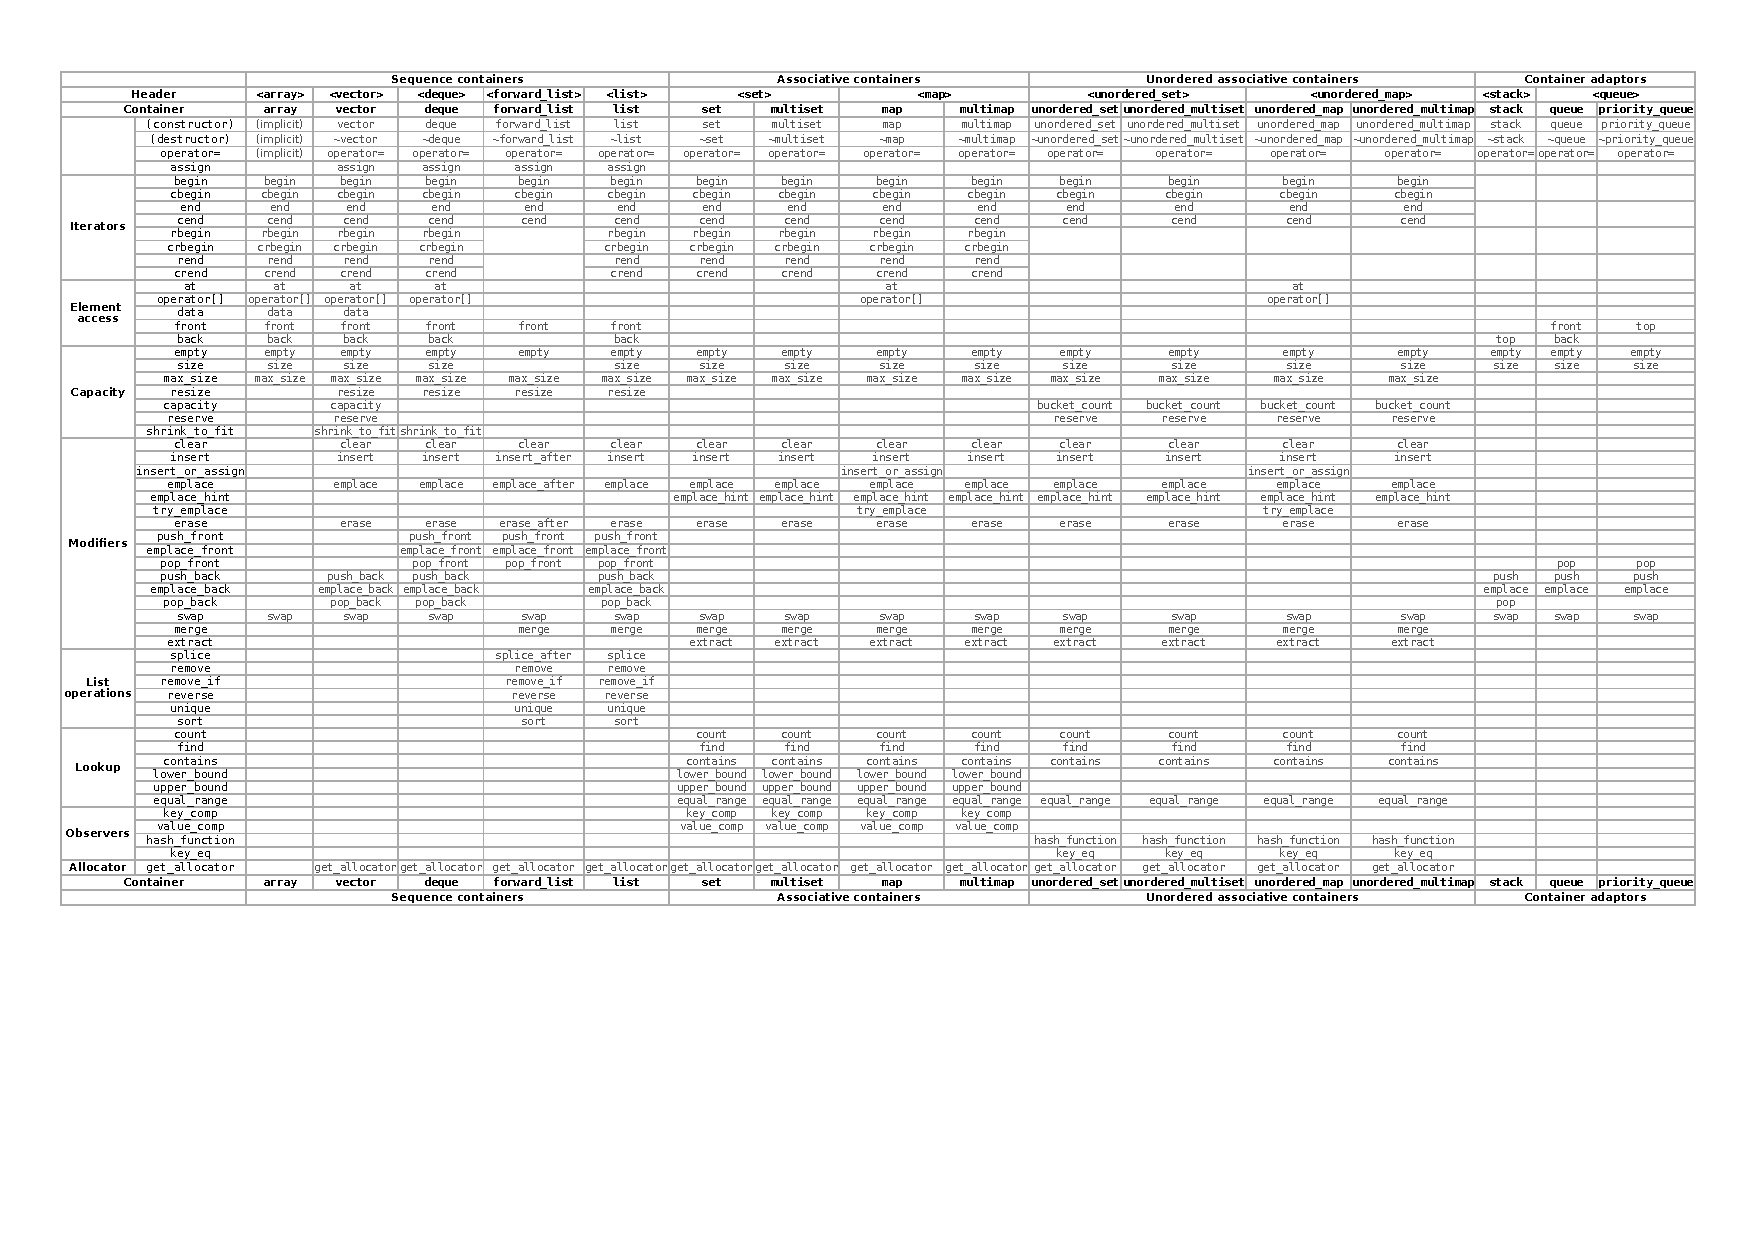
\includepdf[angle=270]{others/stl.pdf}
	\else
		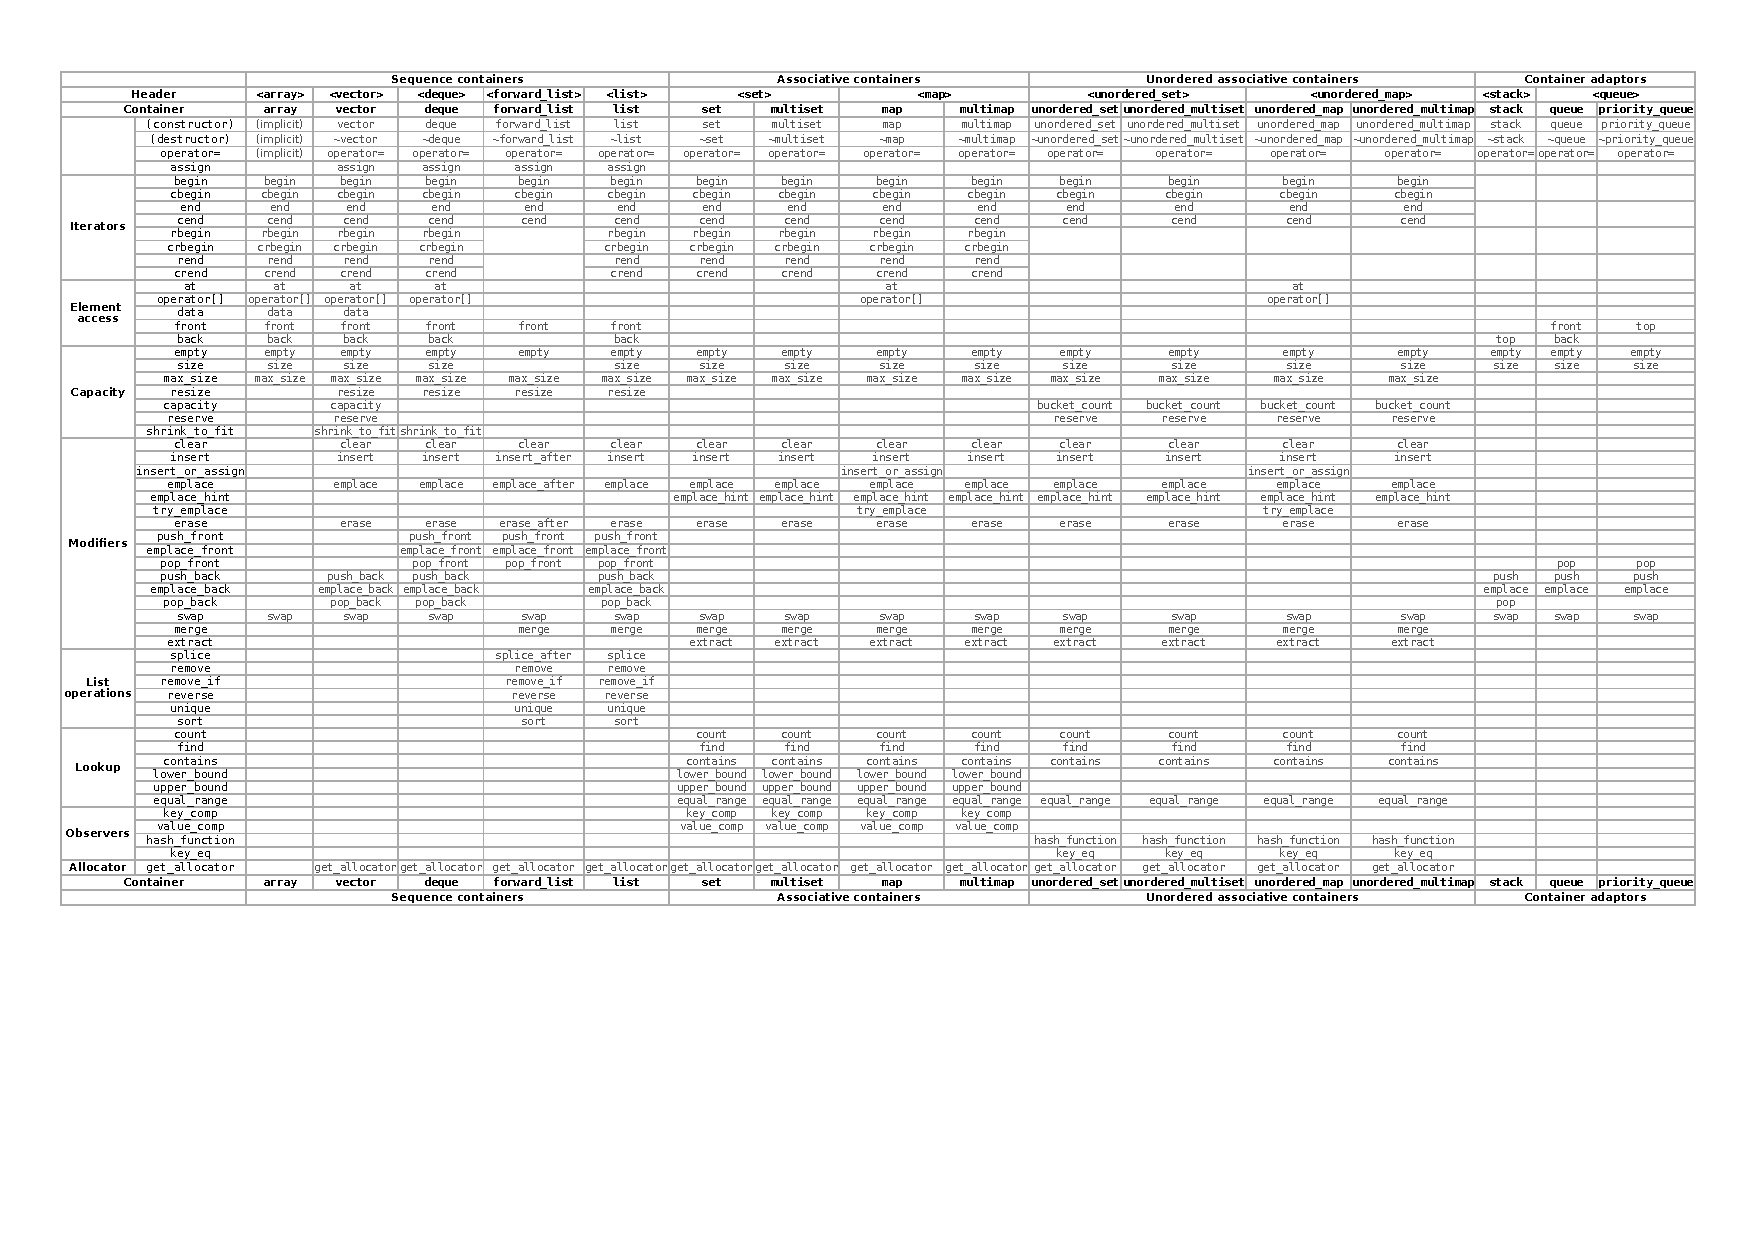
\includepdf[angle=90]{others/stl.pdf}
	\fi
